%%%
% Plantilla de Presentación
% Modificación de una plantilla de Latex de LaTeXTemplates para adaptarla 
% al castellano y a las necesidades de escribir informática y matemáticas.
%
% Editada por: Mario Román
%
% License:
% CC BY-NC-SA 3.0 (http://creativecommons.org/licenses/by-nc-sa/3.0/)
%%%

%%%%%%%%%%%%%%%%%%%%%%%%%%%%%%%%%%%%%%%%%
% Beamer Presentation
% LaTeX Template
% Version 1.0 (10/11/12)
%
% This template has been downloaded from:
% http://www.LaTeXTemplates.com
%
% License:
% CC BY-NC-SA 3.0 (http://creativecommons.org/licenses/by-nc-sa/3.0/)
%
%%%%%%%%%%%%%%%%%%%%%%%%%%%%%%%%%%%%%%%%%

%----------------------------------------------------------------------------------------
%	PAQUETES Y CONFIGURACIÓN DEL DOCUMENTO
%----------------------------------------------------------------------------------------

\documentclass{beamer}

%% Configuración de la presentación
\mode<presentation> {
  %%% Selección de estilo
  % The Beamer class comes with a number of default slide themes
  % which change the colors and layouts of slides. Below this is a list
  % of all the themes, uncomment each in turn to see what they look like.

  %\usetheme{default}
  %\usetheme{AnnArbor}
  %\usetheme{Antibes}
  %\usetheme{Bergen}
  %\usetheme{Berkeley}
  %\usetheme{Berlin}
  %\usetheme{Boadilla}
  %\usetheme{CambridgeUS}
  %\usetheme{Copenhagen}
  %\usetheme{Darmstadt}
  %\usetheme{Dresden}
  %\usetheme{Frankfurt}
  %\usetheme{Goettingen}
  %\usetheme{Hannover}
  %\usetheme{Ilmenau}
  %\usetheme{JuanLesPins}
  %\usetheme{Luebeck}
  \usetheme{Madrid}
  %\usetheme{Malmoe}
  %\usetheme{Marburg}
  %\usetheme{Montpellier}
  %\usetheme{PaloAlto}
  %\usetheme{Pittsburgh}
  %\usetheme{Rochester}
  %\usetheme{Singapore}
  %\usetheme{Szeged}
  %\usetheme{Warsaw}

  %% Selección de color
  % As well as themes, the Beamer class has a number of color themes
  % for any slide theme. Uncomment each of these in turn to see how it
  % changes the colors of your current slide theme.

  %\usecolortheme{albatross}
  %\usecolortheme{beaver}
  %\usecolortheme{beetle}
  %\usecolortheme{crane}
  %\usecolortheme{dolphin}
  %\usecolortheme{dove}
  %\usecolortheme{fly}
  %\usecolortheme{lily}
  %\usecolortheme{orchid}
  %\usecolortheme{rose}
  %\usecolortheme{seagull}
  %\usecolortheme{seahorse}
  %\usecolortheme{whale}
  %\usecolortheme{wolverine}

  %% Configuración del pie de línea
  %\setbeamertemplate{footline} % To remove the footer line in all slides uncomment this line
  %\setbeamertemplate{footline}[page number] % To replace the footer line in all slides with a simple slide count uncomment this line
  %\setbeamertemplate{navigation symbols}{} % To remove the navigation symbols from the bottom of all slides uncomment this line
}

%% Fuentes de tamaño arbitrario
\usepackage{lmodern}

%% Gráficos
\usepackage{graphicx} % Allows including images
\usepackage{booktabs} % Allows the use of \toprule, \midrule and \bottomrule in tables

%%% Castellano.
% noquoting: Permite uso de comillas no españolas.
% lcroman: Permite la enumeración con numerales romanos en minúscula.
% fontenc: Usa la fuente completa para que pueda copiarse correctamente del pdf.
\usepackage[spanish,es-noquoting,es-lcroman]{babel}
\usepackage[utf8]{inputenc}
\usepackage[T1]{fontenc}
\selectlanguage{spanish}

%----------------------------------------------------------------------------------------
%	TÍTULO
%----------------------------------------------------------------------------------------

\title[Protocolo SIP y VoIP]{Protocolo SIP y VoIP} % The short title appears at the bottom of every slide, the full title is only on the title page

\author{Óscar Bermúdez, Lothar Soto} % Your name
\institute[UGR] % Your institution as it will appear on the bottom of every slide, may be shorthand to save space
{
  Universidad de Granada \\ % Your institution for the title page
  \medskip
  \textit{lsotpal@correo.ugr.es\\
  oscarbg@correo.ugr.es} % Your email address
}
\date{\today} % Date, can be changed to a custom date



\begin{document}

%% Diapositiva de título.
\begin{frame}
\titlepage % Print the title page as the first slide
\end{frame}

%% Diapositiva de contenidos.
% Throughout your presentation, if you choose to use \section{} and \subsection{} commands, 
% these will automatically be printed on this slide as an overview of your presentation
\begin{frame}
  \frametitle{Contenidos} % Table of contents slide, comment this block out to remove it
  \tableofcontents
\end{frame}



%----------------------------------------------------------------------------------------
%	PRESENTACIÓN
%----------------------------------------------------------------------------------------

%------------------------------------------------
\section{SIP} % Sections can be created in order to organize your presentation into discrete blocks, all sections and subsections are automatically printed in the table of contents as an overview of the talk
%------------------------------------------------

	\subsection{Un poco de historia} % A subsection can be created just before a set of slides with a common theme to further break down your presentation into chunks
	\begin{frame}
	\frametitle{Un poco de historia}
		SIP o Protocolo de Inicio de Sesiones es un protocolo desarrollado por el \textbf{IETF MMUSIC Working Group} con la intención de ser el estándar para la iniciación, modificación y finalización de sesiones interactivas de usuario donde intervienen elementos multimedia.
		
		Puede funcionar en Transmission Control Protocol(\textbf{TCP}), User Datagram Protocol(\textbf{UDP}) o Stream Control Transmission Protocol(\textbf{SCTP}).\\~\\
		Fue publicado en:
		\begin{itemize}
		\item RFC-2543, RFC-3261.
		\end{itemize}
	\end{frame}
	
	\subsection{Funcionalidades}
	\begin{frame}
	\frametitle{Especificación, Modificación y fin de sesión}
		El estándar SIP define la forma en la que se lleva a cabo el establecimiento, modificación y el fin de comunicación multimedia. \\~\\
		Para iniciar un proceso de comunicación es necesario que:
		\begin{itemize}
			\item El usuario añadido al proceso acepte participar en dicha sesión.
			\item Los usuarios establezcan los parámetros multimedia a utilizar.\\~\\
		\end{itemize}
	\end{frame}
	
	\begin{frame}
	\frametitle{Funcionalidad}
		El funcionamiento de SIP se realiza de la siguiente forma:
		\begin{itemize}
			\item Los usuarios establecen los códec de voz y vídeo a usar u otros parámetros multimedia.
			\item Si se producen cambios durante la comunicación, se notifican a los usuarios que formen parte de la misma.
			\item Por último, en el momento en el que uno de los usuarios desea llevar a cabo la desconexión, se notifica al resto de usuarios de la misma.
		\end{itemize}
	\end{frame}
	
	\begin{frame}
	\frametitle{Movilidad}
		Una de las más importantes ventajas de la telefonía IP es que se puede usar el servicio sin necesidad de encontrarse en una red específica. El protocolo SIP, antes de realizar la comunicación entre usuarios, requiere del reconocimiento de la dirección IP.\\~\\
		Herramientas que usa:
		\begin{description}
			\item[-]\textbf{URL SIP:} Se le asigna una URL a cada usuario de la red con el objetivo de dar una referencia única en internet. Tiene el siguiente formato:\\
			\begin{example}[URL SIP:]
				SIP://<user>:<password>@<host><tlf>:<PORT>
			\end{example}
	
			\item[-]\textbf{Registros:} Esto permite al usuario cambiar su ubicación en lo que a dirección IP.
		\end{description}
	\end{frame}
	
	\subsection{Arquitectura}
	\begin{frame}
	\frametitle{Peticiones}
		\begin{itemize}
			\item \textbf{REGISTER}: Usado por un agente de usuario para registrarse.
			\item \textbf{INVITE}: Usado para establecer una sesión multimedia entre agentes de usuario.
			\item \textbf{ACK}: Confirma que los intercambios de mensajes son confiables.
			\item \textbf{CANCEL}: Cancela una petición pendiente.
			\item \textbf{BYE}: Termina una sesión.
			\item \textbf{OPTIONS}: Solicita información sobre las posibilidades de un agente de usuario sin la necesidad de comenzar una sesión.
		\end{itemize}
	\end{frame}
	
	\begin{frame}
	\frametitle{Respuestas}
		\begin{itemize}
			\item \textbf{Provisional(1xx)}: La petición fue recibida y está siendo  procesada.
			\item \textbf{Success(2xx)}: La acción fue recibida satisfactoriamente, entendida y aceptada.
			\item \textbf{Redirection(3xx)}: Nuevas acciones necesitan ser realizadas para completar la petición.
			\item \textbf{Client Error(4xx)}: La petición tiene un fallo de sintaxis o no puede ser rellenada por el servidor.
			\item \textbf{Server Error(5xx)}: El servidor falló al rellenar una petición aparentemente válida.
			\item \textbf{Global Failure(6xx)}: La petición no puede ser rellenada en ningún servidor.
		\end{itemize}
	\end{frame}
	
	\begin{frame}
	\frametitle{Servidores SIP}
		Un agente de usuario es una entidad de \textbf{SIP} que interactúa con el participante de la sesión. Son aplicaciones que envían y reciben peticiones \textbf{SIP}.
		
		El servidor \textbf{SIP} acepta las peticiones que se realizan para dar una repsuesta. Un servidor \textbf{SIP} se encarga de llevar a cabo funciones que pueden necesitar los distintos agentes de usuario.
		
		Los servidores más usados son:
		\begin{itemize}
			\item Servidor Proxy
			\item Servidor de Localización
			\item Servidor de Redireccionamiento
		\end{itemize}
	\end{frame}
	
	\begin{frame}
	\frametitle{Servidor proxy}
		\begin{figure}
			\centering
			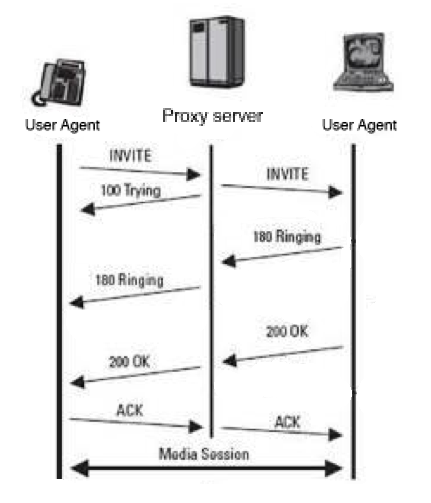
\includegraphics[width=0.5\linewidth]{./Sproxy}\\
			Funcionamiento de un servidor proxy
			\label{fig:Sproxy}
		\end{figure}
	\end{frame}
	
	\begin{frame}
	\frametitle{Servidor de redirección}
		\begin{figure}
			\centering
			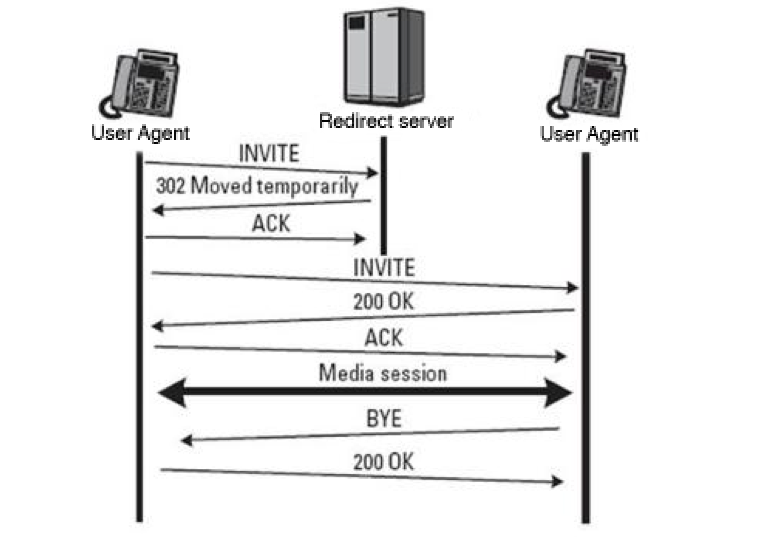
\includegraphics[width=0.7\linewidth]{./Sredirect}\\
			Funcionamiento de un servidor de redirección
			\label{fig:Sredir}
		\end{figure}
	\end{frame}
	
	\subsection{Aplicaciones SIP}
	\begin{frame}
	\frametitle{Aplicaciones SIP}
		SIP define una arquitectura de señalización y control ampliamente para llamadas de voz y vídeo sobre Internet Protocol(VoIP). También puede ser usado para crear, modificar y terminar sesiones de streaming.\\~\\
		Programas que usan SIP son:
		\textbf{\begin{itemize}
			\item OpenWengo
			\item Gizmo Project
			\item Twinkle
			\item Tapioca
			\item KCall
		\end{itemize}}
	\end{frame}

\section{VoIP}
%------------------------------------------------

	\subsection{Funcionamiento}
	\begin{frame}
	\frametitle{Funcionamiento}
		Se digitaliza la voz en paquetes de datos que se envían por la red digitalizadas en señales de pulso(PCM) a través de un codec de voz.\\~\\
		Las muestras PCM se comprimen y se fraccionan en paquetes que pueden ser transmitidos a través de una red.\\~\\
		En el extremo contrario se realizan las mismas operaciones en orden inverso.
	\end{frame}
	
	\subsection{Telefonia IP vs Telefonia convencional}
	\begin{frame}
	\frametitle{Telefonia IP vs Telefonia convencional}
		\begin{tabular}{|p{5.5cm}|p{5.5cm}|}
		\hline
		\textbf{Telefonía convencional} & \textbf{VoIP} \\
		\hline \hline
		Se levanta el teléfono y se conecta con el operador local de telefonía. & Se levanta el teléfono, lo que envía una señal al \textbf{ATA}, y éste envía un tono de llamado. \\
		\hline
		Se marca el número de teléfono. & Se marca el número de teléfono. \\
		\hline
		La llamada es transmitida a través del conmutador(\textbf{switch}) de su operador apuntando hacia el teléfono marcado. & Los datos del número son enviados al proveedor de VoIP para revisar que está en un formato válido. \\
		\hline
		Una conexión es creada entre tu teléfono y el de la persona que estás llamando, entremedio el operador comunica las líneas. & El proveedor determina a quién corresponde este número y lo transforma en una dirección \textbf{IP}. \\
		\hline
		\end{tabular}
	\end{frame}
	
	\begin{frame}
	\frametitle{Telefonia IP vs Telefonia convencional}
		\begin{tabular}{|p{5.5cm}|p{5.5cm}|}
					\hline
			\textbf{Telefonía convencional} & \textbf{VoIP} \\
			\hline \hline
			El teléfono suena y alguien contesta la llamada. & El proveedor conecta los dos dispositivos que intervienen en la llamada y se envía una señal al \textbf{ATA} del receptor para que suene su teléfono. \\
			\hline
			La conexión abre el circuito. & Cuando alguien contesta, se establece una comunicación tu ordenador y el de la otra persona. La infraestructura de internet maneja los paquetes de voz como haría con un email o con una página web. \\
			\hline
		\end{tabular}
	\end{frame}
	
	\begin{frame}
	\frametitle{Telefonia IP vs Telefonia convencional}
		\begin{tabular}{|p{5.5cm}|p{5.5cm}|}
					\hline
			\textbf{Telefonía convencional} & \textbf{VoIP} \\
			\hline \hline
			Uno habla por un tiempo determinado y luego cuelga el teléfono. & Se habla por un periodo de tiempo. Durante la conversación, tu sistema y el del receptor transmiten y reciben paquetes entre sí. \\
			\hline
			Cuando se cuelga el teléfono el circuito automáticamente es cerrado, de esta manera se liberan todas las líneas que intervinieron. & Cuando se termina la llamada, se cuelga el teléfono. En este momento el circuito es cerrado y el \textbf{ATA} envía una señal al proveedor de Telefonía \textbf{IP} informando que la llamada terminó. \\
			\hline
		\end{tabular}
	\end{frame}
	
	\subsection{Características de VoIP}
	\begin{frame}
	\frametitle{Características de VoIP}
		\begin{itemize}
			\item \textbf{Seguridad:} Puesto que el protocolo \textbf{SIP} encripta y autentifica los mensajes de señalización.\\~\\
			\item \textbf{Packet Switched:} Permite el encapsulamiento de datos que serán distribuidos por el medio compartido.\\~\\
			\item \textbf{Operatividad:} Esta tecnología está operativa en cualquier lugar con conexión a la red, pero es necesaria una buena conexión para asegurar la calidad de la llamada.
		\end{itemize}
	\end{frame}	
	
	\subsection{Calidad de servicio (QoS)}
	\begin{frame}
	\frametitle{Calidad de servicio (QoS)}
		QoS es el rendimiento promedio visto por los usuarios de una red de telefonía o de ordenadores. Cuantitativamente, se miden considerando varios aspectos del servicio de red:
		\begin{itemize}
			\item Tasas de errores.
			\item Ancho de banda.
			\item Rendimiento.
			\item Retraso en la transmisión.
			\item Disponibilidad.
			\item Jitter.
			\item Y muchos más.
		\end{itemize}
	\end{frame}
	
	\subsection{Requisitos QoS}
	\begin{frame}
	\frametitle{Retardo o Latencia}
		Establecidos los retardos de tránsito y de procesado de la conversación, la conversación es aceptable si este se encuentra entre los 50 - 150 ms. 
		El retardo puede causar dos problemas principales:
		\begin{itemize}
			\item \textbf{Eco}
			\item \textbf{Pérdida de tramas}:La pérdida de tramas afecta a la calidad de voz dependiendo del modo de gestión de los Frame Erasures que usen los terminales de voz.
		\end{itemize}
	\end{frame}
	
	\begin{frame}
	\frametitle{Jitter}
		Variación de tiempo entre los paquetes causada por la red. Suele considerarse como una señal de ruido, en general como un cambio indeseado y abrupto de la propiedad de una señal. Puede afectar tanto a la amplitud como a la frecuencia o fase.
		Existen distintos tipos:
		\begin{itemize}
			\item Jitter determinista
			\item Jitter aleatorio
			\end{itemize}
	\end{frame}
	
%----------------------------------------------------------------------------------------

\end{document} 